\chapter{Design and Implementation}
This chapter consists of all the design principles that were carried during this project. It also comprises of the machine configurations that were used during the experiments.

\section{Machine Configurations and Programming Languages}
\subsection{Machine Configurations}
Host Machine:
\begin{itemize}
\item Operating System: Windows 8
\item Model: Lenovo Ideapad Z400
\item Processor: Intel(R) Core(TM) i5-3230M CPU @ 2.60 GHz
\item RAM: 6.00 GB
\item System type: 64-bit Operating System, x64 based processor
\end{itemize}

Guest Machine:
\begin{itemize}
\item Operating System: Ubuntu 12.04 LTS
\item Model: Lenovo Ideapad Z400
\item Processor: Intel(R) Core(TM) i5-3230M CPU @ 2.60 GHz
\item RAM: 1.00 GB
\item System type: 64-bit Operating System, x64 based processor
\end{itemize}

\subsection{Programming Languages}
\subsubsection{Java}
\begin{itemize}
\item Java bytecoe manipulation library ASM was used for code obfuscation.
\item Also, Java was used for testing purposes.
\end{itemize}

\subsubsection{Javascript}
\begin{itemize}
\item Javascript was used for creation of sequences and generating Hidden Markov Models.
\end{itemize}

\section{Design}
The metamorphic engine is constructed using the tree API of ASM library. This section will firstly describe the algorithm briefly and then each step of algorithm will be explained in detail. 

\subsection{Algorithm}
The detailed algorithm that is used for design of the morphing code is as follows:
\begin{enumerate}
\item A class MyClassAdapter that inherits ClassNode class in tree package is written. Also, ClassVisitor to read from file, and ClassWWriter is used to write the modified bytecode to the output file.
\item The class MyClassAdapter reads from a file, and makes clone of that class.
\item The main transformation function is used to perform deadcode insertion, subroutine permutation and instruction permutation. 
\begin{enumerate}
\item This function visits the methods in order, transforms it, and then add it to the new cloned class.
\item This method creates two objects, one for insertion of deadcode, and the other for instruction 
permutation. Both these operations are performed in such a way that the overall meaning of the code remains unchanged.
\item The next step performed is subroutine permutation. According to the position of new added methods, the last position of methods is determined. \textit{this.method.add(0, method)} means add new modified method to the front of the method list, so the new cloned class has its methods in reversed order.
\end{enumerate}
\item Once the transformation has been achieved, the last step is to write the class in bytecode format to the output file. The new modified class is written to the output file by the ClassWriter.
\end{enumerate}


As mentioned in Chapter 4, the tree API relies on the use of ClassNode class for generation and transformation of java classes. 

A class can be generated by creating a ClassNode object and  then initializing field values. Class members can be added or removed by addition or removal of elements in the fields or methods of a ClassNode object [21]. 

The ClassNode class extends the ClassVisitor class [21]. The ClassVisitor class provides an accept method, which can be used to generate events depending on the field values of ClassNode.  The ClassVisitor methods performs the opposite operation of setting the ClassNode fields based on the received events. The following code snippet from [21] shows the accept method, along with class hierarchy:

\begin{verbatim}
public class ClassNode extends ClassVisitor {
  ...
    public void visit(int version, int access, String name,
       String signature, String superName, String[] interfaces[]) {
             this.version = version;
             this.access = access;
             this.name = name;
             this.signature = signature;
             ...
    }
  ...
    public void accept(ClassVisitor cv) {
             cv.visit(version, access, name, signature, ...);
             ...
    }
} 
\end{verbatim}


\begin{itemize}
\item Constructing a ClassNode from a byte array can be achieved by combining it with a ClassReader. The events generated by the ClassReader are absorbed by the ClassNode component, which results in the field initialization. The following code snippet from [21] shows how ClassReader can be used: 

\begin{verbatim}
    ClassNode cn = new ClassNode();
    ClassReader cr = new ClassReader(...);
    cr.accept(cn, 0);
\end{verbatim}

\item Similarly, a ClassNode can be converted to its byte array representation by using it with a ClassWriter. In this case, the events generated by the accept method are consumed by the ClassWriter. The code below from [21] shows how ClassWriter is used for converting a ClassNode to its byte representation :

\begin{verbatim}
    ClassWriter cw = new ClassWriter(0);
    cn.accept(cw); 
    byte[] b = cw.toByteArray();

\end{verbatim}

\item Transformation of the classes can be achieved by integrating the ClassReader, the ClassWriter and the addition of transformation code. The transformation code from [21] is :

\begin{verbatim}
    ClassNode cn = new ClassNode(ASM4);
    ClassReader cr = new ClassReader(...);
    cr.accept(cn, 0);
    ...
    // here transform cn as you want
    ClassWriter cw = new ClassWriter(0);
    cn.accept(cw);
    byte[] b = cw.toByteArray();
\end{verbatim}
\end{itemize}



 

\section{Testing}
\subsection{Threshold Approach}
We used Hidden Markov Models to test the obfuscated files. In this approach, we used k-fold cross validation. In our case, we used five-fold cross validation. 100 obfuscated files were divided into five sets of 20 files each. Then four sets were used to create a HMM and the fifth set was tested against this generated HMM. In threshold approach, the HMM is trained using four sets of malware code and tested using fifth subset of malware as well as benign code. Once, we have score for each file, we can decide upon the threshold. If the score is below the threshold, the file is classified as benign. We have performed the testing by using different number of states for HMM. We built 2, 3 and 4 state HMMs for testing.

The table for 2-state HMM testing for malware and benign files is as follows :
\begin{table}
\centering
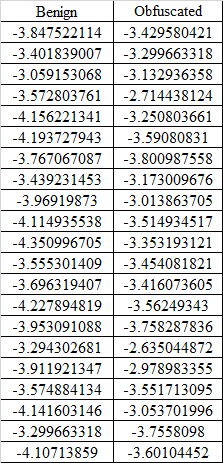
\includegraphics[width=0.5\textwidth]{images/st2_m1.png}
\caption{Table for 2-state model} 
\label{table:Table for 2-state model}
\end{table}

The above results are just results of one slice, i.e. 20 benign files and 20 obfuscated slices tested against obfuscated HMM. Other results using 2,3,4 state models are added in the appendix. Also, it can be seen from above results, that the HMM model correctly classifies the obfuscated files from the benign files. The score for obfuscated file is less than its benign version.  

\subsection{Dueling Approach}
In dueling approach, the HMM is trained for both benign as well as malware datasets. Once, the dataset has been built, the file is scored against each of the HMM, the malware as well as the benign. In this case, the file has multiple scores associated with it. Once, all the scores have been identified, the highest score is checked. If the score is from a malware HMM, the file is classified as malware otherwise, if it from benign HMM, it is classified as benign. 

The table below shows the snapshot of testing, where each benign file is tested against 10 HMMs. The file belongs to that HMM for which it has the highest score. For example, for File 1, the highest score is for benign HMM, m5. Therefore, the file is benign.   

\begin{table}
\centering
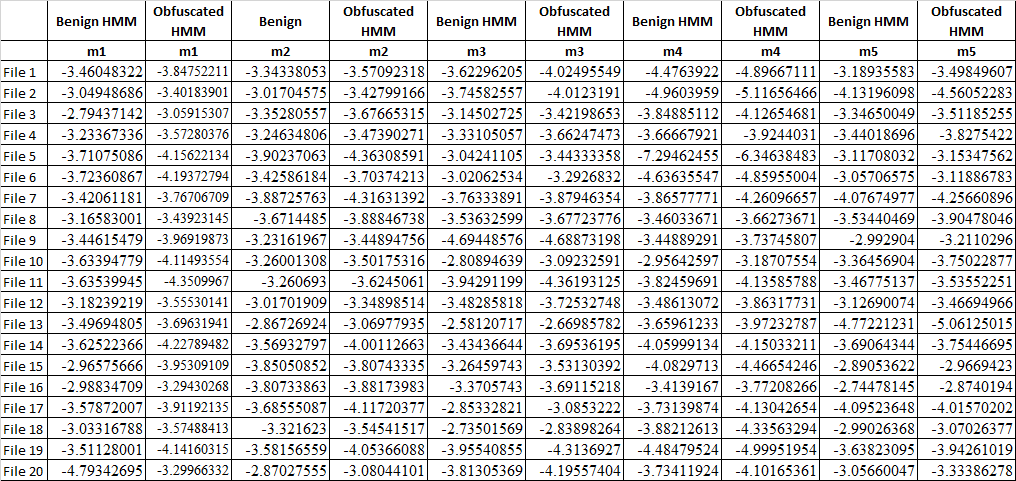
\includegraphics[width=1.0\textwidth]{images/duel.png}
\caption{Table for benign files tested against all 2-state HMMs} 
\label{table:Table for benign files tested against all 2-state HMMs}
\end{table}